\chapter{Discussion}
  \label{sec:discussion}

  \section{Interpretation of Results}
  \label{subsec:interpretation-results}

  This section evaluates the research findings and addresses the five research questions that guided the development of Henshin Web. The evaluation is based on the implementation of a fully functional web-based model transformation editor that demonstrates improvements in accessibility and usability.

  \textbf{RQ1: Web-based Adaptation of Henshin Capabilities} - The implementation demonstrates that adapting Henshin for web environments is both technically feasible and practically achievable through the \ac{glsp} framework. The successful integration of the Henshin \ac{sdk} into the \ac{glsp} server architecture preserves complete transformation functionality while enabling web delivery through Theia Cloud. Converting Eclipse plugins into Maven artifacts enabled to include the Henshin code into the \ac{glsp} project architecture. The three-editor architecture (\code{XMIDiagramModule}, \code{RuleDiagramModule}, \code{EcoreDiagramModule}) successfully handles workflow complexity while maintaining modular design and seamless integration between metamodels, transformation rules, and instance models.

  \textbf{RQ2: Essential Functional Requirements} - The implementation successfully addresses the core use case of creating a metamodel and applying transformation rules to \ac{emf} \ac{xmi} instance files of the metamodel. The identified requirements prove both necessary and sufficient for meaningful model transformation work across stakeholder groups. The integration of rule selection into the Theia explorer enhances workflow efficiency, and undo/redo functionality supports iterative development. The architectural foundation demonstrates scalability for planned enhancements including transformation units and analysis capabilities.

  \textbf{RQ3: Accessibility and User Experience Improvements} - The web-based approach demonstrates accessibility improvements. Eliminating Eclipse installation requirements enables browser-based access without complex environment setup, particularly benefiting new users of Henshin. The graphical interface based on \ac{glsp} and Theia principles provides more intuitive experiences than the graphical editor of Eclipse and tree-based editors. Cross-platform accessibility and consistent visual representation reduce learning curves. Direct integration of transformation application into the instance editor improves workflow efficiency compared to Eclipse wizard-based approach.

  \textbf{RQ4: Deployment Strategy Impact} - The evaluation of multiple deployment options reveals that Theia Cloud proves most effective for maximizing accessibility. The cloud-based approach eliminates installation requirements while providing consistent performance and enterprise-ready capabilities. Trade-offs between Docker containers (local file access vs. installation complexity) and Electron applications (no browser dependency vs. installation requirements) highlight the advantages of the cloud approach. The Kubernetes infrastructure with automatic scaling addresses performance concerns while infrastructure-as-code ensures reproducible deployments.

  \textbf{RQ5: EMF and Henshin Ecosystem Integration} - The implementation demonstrates comprehensive compatibility with existing ecosystems. Direct use of \ac{emf} data structures ensures complete compatibility with existing files, while \code{EMFSourceModelStorage} integration preserves metadata and relationships for seamless round-trip editing. Although notation files use different formats, semantic content remains fully compatible. Existing Projects can be easily migrated byy just copying the files into the Theia editor. The Henshin \ac{sdk} integration preserves complete transformation semantics, ensuring identical results between web and Eclipse environments. The modular architecture supports future integration while providing value as an independent tool.

  \section{Challenges and Limitations}
  \label{subsec:challenges-limitations}

  While Henshin Web demonstrates significant progress toward accessible model transformation tools, several challenges emerged during development and certain limitations constrain the system's capabilities compared to the mature Eclipse Henshin plugin.

  \textbf{Technical Integration Challenges} - The integration of Henshin into \ac{glsp} presented substantial challenges. Bridging the architectural gap between Eclipse plugin-based and Maven-based development required creating a custom packaging system to convert the Henshin Eclipse plugins into Maven artifacts. This introduces maintenance overhead for future Henshin versions. The indexing of \ac{emf} models proved complex, requiring different strategies for each model type: Henshin rules (existing identifiers), Ecore metamodels (UUIDs and content hashes), and \ac{xmi} instances (adapters and content hashes). Notation model synchronization presents ongoing challenges, particularly the content-hash approach for \ac{xmi} instances requiring frequent updates.

  \textbf{Functional Limitations} - The current implementation focuses on core functionality, leaving advanced features unavailable compared to the full Eclipse plugin. Missing capabilities include transformation units for complex scenarios, the usage of JavaScript variables, state space analysis, conflict detection, and comprehensive debugging tools. The web environment constraints prevent integration of step-through debugging capabilities that Eclipse provides. Collaborative editing features are not yet implemented, limiting team-based development scenarios.

  \textbf{Ecosystem and User Experience Limitations} - Although users are not required to install an \acs{ide}, registration is necessary to use Henshin Web. While maintaining file format compatibility, the system lacks seamless integration with the broader Eclipse modeling ecosystem. Tools depending on Eclipse platform services cannot be directly integrated. Henshin Web allows the extension of  different \ac{mde} use cases in the future, but they have to be develop explicitly. Notation model format differences require conversion when moving between environments. Cloud deployment requires file upload/download, creating workflow friction compared to direct file system access. Current English-only interface limits international adoption.

  \section{Summary of Contributions}
  \label{subsec:summary-contributions}

  The primary contribution of this thesis is the successful creation of a working, full web-based model transformation application that significantly reduces barriers to entry model transformations with Henshin while maintaining complete functional compatibility with the established Eclipse-based ecosystem. Henshin Web demonstrates that model transformation capabilities can be made accessible through modern web technologies without sacrificing the computational integrity or ecosystem compatibility that characterizes the Eclipse Henshin plugin. The application enables users to create metamodels, define transformation rules, and apply transformations to instance models entirely through a web browser without requiring Eclipse installation, plugin configuration, or local development environment setup. By preserving the complete Henshin Java \ac{sdk} functionality and maintaining full compatibility with existing \ac{emf} Ecore metamodels, \ac{xmi} instance files, and Henshin transformation rules, the web-based implementation ensures that users can seamlessly transition between Eclipse-based and web-based workflows while benefiting from improved accessibility and user experience. The three-module architecture built on the \ac{glsp} framework provides a robust foundation for graphical editing of interconnected model types, while the cloud-based deployment through Theia Cloud eliminates traditional adoption barriers and enables immediate access to model transformation capabilities for students, researchers, and software engineers without compromising the functional depth that makes Henshin valuable for production use cases. 

  \section{Suggestions for Future Development}
  \label{subsec:suggestions-future-development}

  The foundation established by Henshin Web provides numerous opportunities for enhancement and extension. Future development efforts should focus on expanding transformation capabilities, improving collaborative features, and integrating additional modeling tools to establish Henshin Web as a comprehensive platform for model-driven engineering.

 \textbf{Complete Henshin Functionality Implementation} - The current implementation should be systematically extended with the complete Henshin feature set. Transformation units would support sequential, conditional, and iterative rule applications through flowchart-like graphical interfaces for designing complex transformation workflows. State space analysis functionality would enable interactive visualization of transformation paths and resulting models. Conflict and dependency analysis would highlight conflicting rules and visualize dependency relationships. Advanced debugging capabilities should include step-through execution, inspection of intermediate states, and detailed logging with debugging views showing current transformation state, matched elements, and parameter bindings.
 
  \textbf{Edapt Integration for Model Evolution} - An ongoing problem is the adaption of instance files after updating the Ecore metamodel. The integration of Edapt (EMF Adaptation) \cite{edapt-repo}provides systematic support for model evolution and migration, addressing the common challenge of maintaining instance models when metamodels change. This integration would involve extending the \code{EcoreDiagramModule} to include Edapt's difference detection algorithms and migration rule generation. Since a Henshin Web projects often contains multiple instance files, that should always be in sync with the metamodel, inconsistencies may arise when the instance files are not updated after metamodel changes. Edapt can help to overfome these inconsistencies by automatically migrating the instance files without requiring manual intervention from the user and without custom migration scripts.

  \textbf{Collaborative Modeling Capabilities} -  Real-time collaborative editing would transform Henshin Web into a platform for team-based model transformation development. \ac{glsp} provides a real-time synchronous diagram collaboration extension \cite{glsp-collab} that is comatible with the existing architecture and Eclipse Theia. It can be integrated into Henshin Web to enable multiple users to collaboratively edit metamodels, transformation rules, and instance models simultaneously, enhancing teamwork and knowledge sharing. It can be used without major architectural changes because one user acts as a coordinator communicating with the \ac{glsp} server, as shown in Figure \ref{fig:glsp-collaboration}.

  \begin{figure}
    \centering
    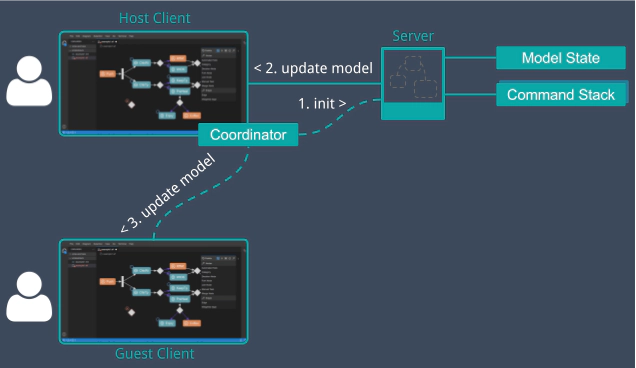
\includegraphics[width=0.7\textwidth]{images/glsp-collab}
    \caption{GLSP Real-Time Collaboration Extension \cite{glsp-collab}}
    \label{fig:glsp-collaboration}
  \end{figure}

  \textbf{Extension with Additional Modeling Tools} - Future development should integrate Henshin Web with the broader MDE ecosystem. Code generation capabilities would extend utility beyond transformation to complete development workflows, allowing users to define generation templates and apply them to transformed models. Integration with model validation frameworks would enable constraint checking, completeness analysis, and semantic validation directly within the web interface. Therefore, Henshin Web can be used as a architectural template for various \ac{mde} use cases in the future.